\documentclass[t,xcolor={usenames,dvipsnames}]{beamer}

\mode<presentation>
{
\usetheme{Frankfurt}%{Warsaw}
%\setbeamercovered{transparent}
%\setbeamercolor{background canvas}{bg=white}
}

% Delete these, if you do not want the table of contents to pop up at
% the beginning of each (sub)section:
%\AtBeginSubsection[]
%{
%  \begin{frame}<beamer>{Outline}
%    \tableofcontents[currentsection,currentsubsection]
%  \end{frame}
%}
%\AtBeginSection[]
%{
%  \begin{frame}<beamer>{Outline}
%    \tableofcontents[currentsection]
%  \end{frame}
%}

\usepackage[english]{babel}
\usepackage[latin1]{inputenc}
\usepackage{times}
\usepackage[T1]{fontenc}
\usepackage{verbatim}
\usepackage{url}
\usepackage{amsmath,amssymb}
\usepackage{comment}
\usepackage[overlay,absolute]{textpos}
\usepackage{hyperref}

% Author-date citations
\usepackage[authoryear,round]{natbib}
\let\cite=\citep  % default \cite such as {\LaTeX} authors are used to

% Where \includegraphics should look for figures
\graphicspath{{./figs/}{../group_talk_2011_11_29/figs/}}
\usepackage{epstopdf}
\DeclareGraphicsExtensions{.eps,.png,.jpg,.pdf}

% Shortcuts
\newcommand{\myhref}[2]{\href{#1}{\textcolor{Blue}{#2}}}
\newcommand{\myurl}[1]{\myhref{#1}{#1}}
\newcommand{\subitem}[1]{\begin{itemize}[<.->]\item #1 \end{itemize}}
\newcommand{\ghead}[1]{{\tiny #1\\}}
\newcommand{\doi}[1]{\myhref{http://dx.doi.org/#1}{doi:#1}}
\newcommand{\csym}[1]{\textcolor{Blue}{\texttt{#1}}}
\newcommand{\ud}{\mathrm{d}}
\newcommand{\dt}{\ud t}

%%%%%%%%%%%%%%%%%%%%%%%%%%%%%%%%%%%%%%%%%%%%%%%%%%%%%%%%%%%%%%%%%%%%%%
\title{Functional Curation}
\author{Jonathan Cooper}
\institute[University of Oxford]
{Computational Biology Group\\
 Department of Computer Science\\
 University of Oxford}
\date{April 14, 2014}

\begin{document}

\begin{frame}
\titlepage
\end{frame}

\begin{comment}
This talk is just a brief intro/reminder of functional curation, before
giving a demo of the website.
\end{comment}

%%%%%%%%%%%%%%%%%%%%%%%%%%%%%%%%%%%%%%%%%%%%%%%%%%%%%%%%%%%%%%%%%%%%%%

%\begin{frame}{Outline}
%\setcounter{tocdepth}{1}
%\tableofcontents
%\end{frame}

%%%%%%%%%%%%%%%%%%%%%%%%%%%%%%%%%%%%%%%%%%%%%%%%%%%%%%%%%%%%%%%%%%%%%%
\section{Motivation}
\subsection*{Main}
%%%%%%%%%%%%%%%%%%%%%%%%%%%%%%%%%%%%%%%%%%%%%%%%%%%%%%%%%%%%%%%%%%%%%%

\begin{frame}{Modelling biology}
\begin{itemize}
\item A mathematical model encodes a quantitative hypothesis about a biological system
\item It can be used to make predictions about the response of the system to experiments
  \subitem{``If I make this intervention, I expect to see that change''}
\item Increasingly, models build on previously published models
  \begin{itemize}
  \item Compose models together to study larger system
    % examples: reaction networks, nephrons/kidneys, heart
  \item Extend or modify models to incorporate latest understanding, or look at effect of disease / drug / species / age / \ldots
  \end{itemize}
\end{itemize}
\end{frame}


\begin{frame}{Using models}
\begin{itemize}
\item As hypothesis encodings, models are developed \emph{for a specific purpose}
  \subitem{May not be appropriate for studying same system in different context}
\item How can we\ldots
  \begin{itemize}
  \item determine a model's functionality, i.e.\ its suitability or limitations for a new study?
  \item re-use a model in a different experimental context?
  \item compare hypotheses: different models' behaviours under the same experiment?
  \end{itemize}
\end{itemize}
\end{frame}


\begin{frame}{Prior state-of-the-art}
\begin{itemize}
\item 264 CellML models / model variants for electrophysiology --- very good thing!
\item Top level of CellML curation is usually that someone has attempted to reproduce one? / some? / all? of the graphs in a paper
\item Even IF the model is a perfect representation of the published model\ldots
  \begin{itemize}
  \item \ldots we still didn't know whether to trust it for doing science!
  \item We still couldn't automatically display the results of even the protocol hardcoded in the model % TODO: Get Alan to check this!
  \item This is where the idea of `Functional Curation' --- examining the behaviour of a model in different situations --- comes in
  \end{itemize}
\end{itemize}
\end{frame}


%%%%%%%%%%%%%%%%%%%%%%%%%%%%%%%%%%%%%%%%%%%%%%%%%%%%%%%%%%%%%%%%%%%%%%
\section{Functional curation with virtual experiments}
\subsection*{Main}
%%%%%%%%%%%%%%%%%%%%%%%%%%%%%%%%%%%%%%%%%%%%%%%%%%%%%%%%%%%%%%%%%%%%%%

\begin{frame}{The essence}
\subitem{Separate \alert{model structure} and \alert{experimental scenario}}
\vspace{-.2cm}
\hspace{-1cm}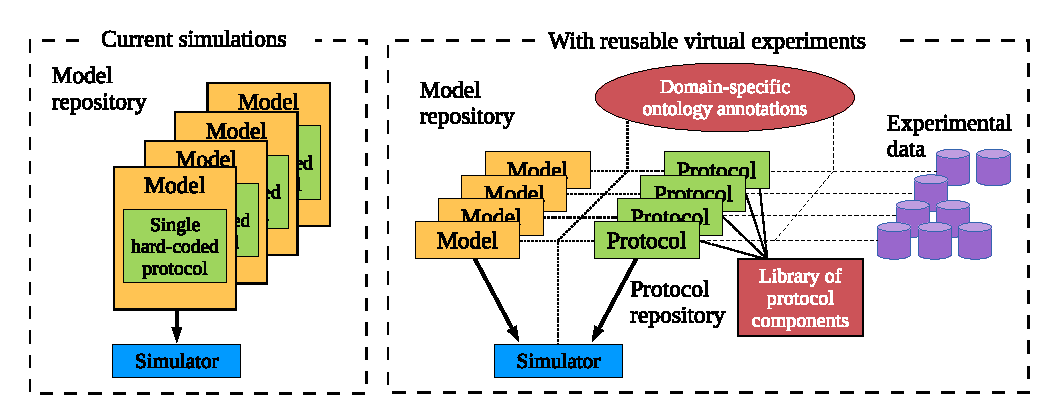
\includegraphics[width=1.185\textwidth]{virtual_expts_schematic}
\vspace{-.31cm}
\begin{itemize}
\item Apply any \alert{virtual experiment} to any (relevant) model
\item One definitive version of each model / protocol
\item Automatically generate post-processed outputs, plots, etc.
\end{itemize}
\end{frame}


%%%%%%%%%%%%%%%%%%%%%%%%%%%%%%%%%%%%%%%%%%%%%%%%%%%%%%%%%%%%%%%%%%%%%%
\section{Demo}
\subsection*{Main}
%%%%%%%%%%%%%%%%%%%%%%%%%%%%%%%%%%%%%%%%%%%%%%%%%%%%%%%%%%%%%%%%%%%%%%

\begin{frame}{Exemplar system: Cardiac electrophysiology!}
\begin{center}
\vspace{-.5cm}
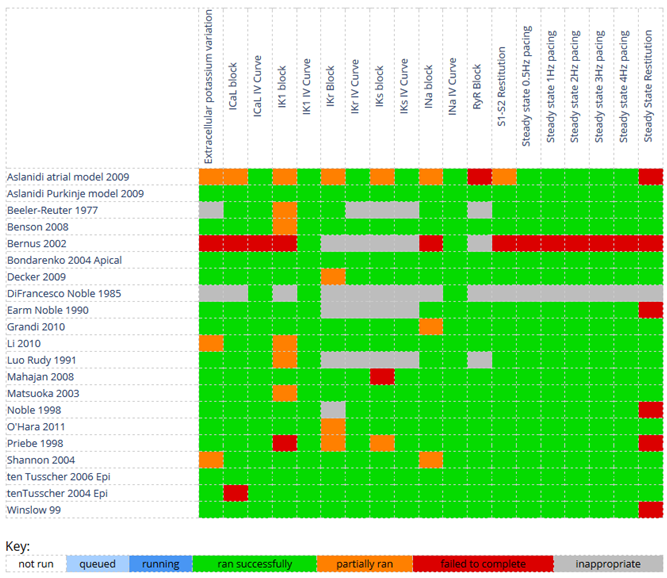
\includegraphics[height=.8\textheight]{cardiac_fc_matrix}\\
\myurl{https://chaste.cs.ox.ac.uk/FunctionalCuration}
\end{center}
\end{frame}


\begin{comment}
\begin{frame}{Live demo}
\begin{itemize}
\item Start at front page of site, and explain things you can do
\item Upload a new annotated model and run all protocols on it - show results at end!
\item Display a single experiment result, e.g.\ ten Tusscher 2006 action potential for 1Hz steady pacing
\item Compare models under a single protocol
  \begin{itemize}
  \item Priebe, ten Tusscher(s), Matsuoka, Grandi, O'Hara (human models) under 2Hz pacing
  \item All models under IK1 block: default plot, then resting potential
  \end{itemize}
\item Compare protocols for a single model: e.g.\ O'Hara at different pacing rates, and then different restitution curves (note alternans at high frequency)
\end{itemize}
\end{frame}
\end{comment}

%%%%%%%%%%%%%%%%%%%%%%%%%%%%%%%%%%%%%%%%%%%%%%%%%%%%%%%%%%%%%%%%%%%%%%
\section{Conclusions}
\subsection*{Main}
%%%%%%%%%%%%%%%%%%%%%%%%%%%%%%%%%%%%%%%%%%%%%%%%%%%%%%%%%%%%%%%%%%%%%%

\begin{frame}{Goals of this work}
\begin{itemize}[<+->]
\item Provide a framework for a coherent approach to model fitting, simulation, comparison and validation
  \begin{itemize}[<.->]
  \item Continuous evaluation of model predictions against experimental data, throughout model lifecycle
  \item Models that are robust, well tested, and well characterised for particular biological studies
  \item Model development akin to high quality software
  \item Improve model reuse and simulation result reproducibility
  \end{itemize}
\item A functional curation system \alert{for each domain}
  \begin{itemize}[<.->]
  \item Brings together competing models, experimental data, and virtual experiments
  \item New models, experiments, or data analysed automatically under all relevant combinations
  \only<3>{\item \alert{A crucial part of a researcher's toolkit}}
  \end{itemize}
\end{itemize}
\end{frame}


\begin{frame}{Areas for community engagement}
%Talk about what the CellML / PMR projects could do to integrate with this; easy wins etc.
\begin{itemize}
\item Linking between models and protocols requires agreement on terms used to annotate models
  \begin{itemize}
  \item Develop a community standard ontology to use for the cardiac case
  \item Provide annotated models direct from the CellML repository
  \end{itemize}
\item Develop a protocol editor as an OpenCOR plugin, facilitating the creation of new protocols
\item Incorporate protocol language features in future versions of SED-ML
\item Ultimately, functional curation systems should be embedded between model repositories and experimental databases
\end{itemize}
\end{frame}


\begin{frame}{A vision of the future}
\begin{itemize}
\item \textbf{With this work}: we know which models are sensible to use for which studies
\item \textbf{With this work}: we can publish protocols with models, to immediately allow reproduction of graphs in a paper
\item Future: experimental data come with a machine-readable protocol description
\item Future: models are auto-checked against new data
\item Future: models are auto-updated by fitting to new data
\item Future: models are auto-developed to take into account latest findings
\end{itemize}
\end{frame}


%%%%%%%%%%%%%%%%%%%%%%%%%%%%%%%%%%%%%%%%%%%%%%%%%%%%%%%%%%%%%%%%%%%%%%
\begin{frame}{Acknowledgments}
Gary Mirams, Erich Kerekes, Martin Scharm, Aidan Daly\\
Chaste team\\
Alan Garny, Steven Niederer, David Gavaghan

Reference publication: \doi{10.1016/j.pbiomolbio.2011.06.003}\\
Website: \myurl{https://chaste.cs.ox.ac.uk/FunctionalCuration}

\begin{center}

\includegraphics[scale=.9]{chaste-266x60}\\ \vspace{.3cm}

\includegraphics[scale=.7]{logo2020science}\\ \vspace{.4cm}

\includegraphics[width=.55\textwidth]{EPSRC1RGBLO} \hspace{.1cm}

\includegraphics[scale=.55]{logo_msr}
\end{center}
\end{frame}


%%%%%%%%%%%%%%%%%%%%%%%%%%%%%%%%%%%%%%%%%%%%%%%%%%%%%%%%%%%%%%%%%%%%%%
\appendix

\begin{frame}{Appendix}
Further information slides follow \dots
\end{frame}

\begin{frame}{Our protocol structure}
\begin{center}
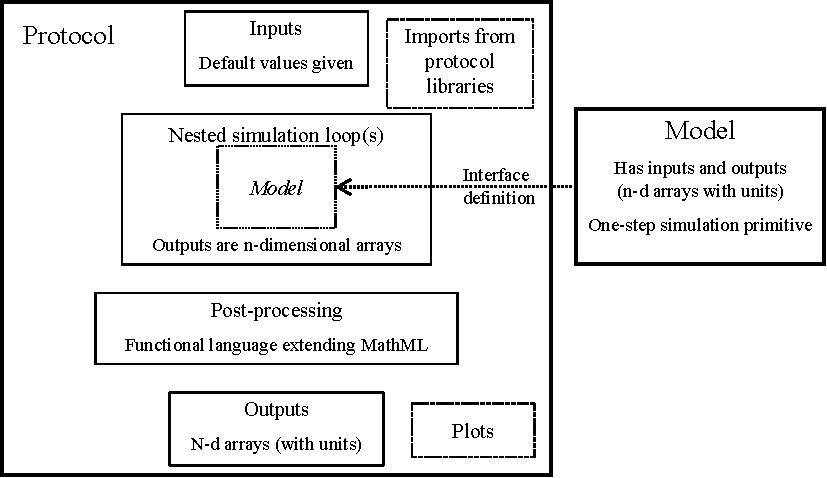
\includegraphics[width=\textwidth]{protocol_language}
\end{center}
\end{frame}

\begin{frame}{What goes in a protocol?}
\begin{itemize}
\item Definition of the interface with the model being experimented on
  \begin{itemize}
  \item Handle variations in modelling conventions: naming, encoding the biology in mathematics
  \item Units conversions
  \item Isolate relevant sub-model(s), using model inputs \& outputs of interest
  \end{itemize}
\item Definition of simulations to perform
\item Post-processing operations on simulation results
\item Description of what to plot
\vspace{.5cm}
\item Also language features facilitating building complex protocols, e.g.\ protocol inputs, outputs, and imports.
\end{itemize}
\end{frame}


\begin{frame}{Challenges arising from cell-based work}
\begin{itemize}
\item Setting `biological' parameters that don't have direct representations in all models
  \subitem{Or vary spatially}
\item Describing the coupling of component models
\item Cell birth \& death imply non-regular result arrays
  \subitem{Increases technical complexity of post-processing}
\item What post-processing should be in the protocol language?
  \begin{itemize}[<.->]
  \item What is best as dedicated code or workflow?
  \item A language targeted at protocol exchange should be supportable by multiple tools
  \item Contrast: rapid prototyping, or deposition in a repository of standard experiments
  \end{itemize}
\end{itemize}
\end{frame}

\end{document}
